\documentclass[11pt,a4paper,titlepage]{article}

\usepackage{pdflscape}
\usepackage[margin=1in]{geometry}
\usepackage{titling}
\usepackage{graphicx}
\usepackage{titlesec}
\usepackage[hidelinks]{hyperref} 

\graphicspath{ {./Images/} }

\setcounter{secnumdepth}{4}

\titleformat{\paragraph}
{\normalfont\normalsize\bfseries}{\theparagraph}{1em}{}
\titlespacing*{\paragraph}
{0pt}{3.25ex plus 1ex minus .2ex}{1.5ex plus .2ex}

\begin{document}
%\title{ \huge Functional Requirements for the SAMBUG}

\begin{titlepage}
	
	
	\begin{center}
		\vspace*{-3cm}
  		\makebox[\textwidth]{
\includegraphics[width=\paperwidth]{sambug}}
	\end{center}
	
	%
\includegraphics[width=\paperwidth]{sambug}
	
    \centering
    \vfill
    {\bfseries\Huge
    \vspace*{-3cm}
         User Manual for the SAMBUG System\\
      \hfill\\
         \Large Subtrop
        \vskip2cm
    }        
    
    \textbf{July, 2015}
    \vfill
\end{titlepage}
	
	

\tableofcontents

\pagebreak

\section{System Overview}

\section{System Configuration}

\section{Installation}
		
\section{Getting started}

\section{Using the system}

\section{Troubleshooting}

\end{document}

%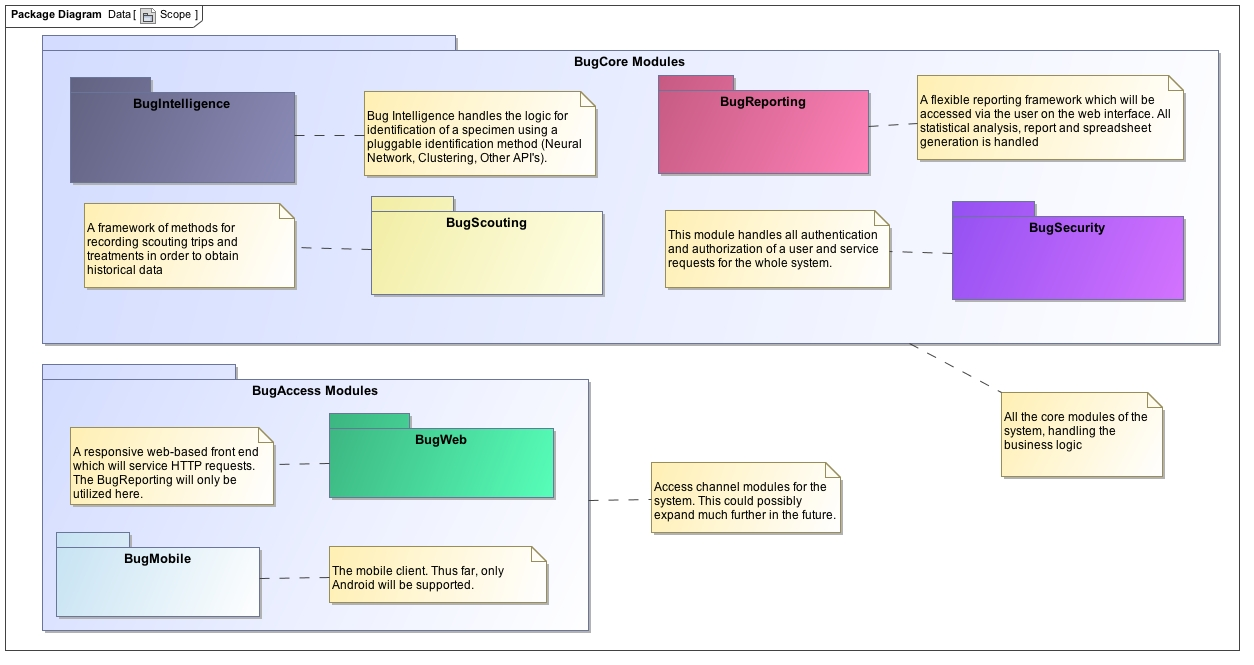
\includegraphics[width=\linewidth]{scope}